\chapter{Empirical study}
\label{ch:empirical-study}

In this chapter the previously proposed physical data models for MongoDB and Neo4j are implemented and put to the test.
A Ruby on Rails application was developed that uses Mongoid and Neo4j.rb libraries to provide connectivity to the data stores.
Custom benchmarking scripts were implemented using the RSpec library \autocite{RSpec2005} and the \texttt{Benchmark} class built into the Ruby implementation.

\section{Previous work}
\label{sec:previous-work}

% Netflix benchmark, http://www.bgbenchmark.org/BG/, XGDBench

In current literature there are already some studies present that compare NoSQL data stores based on a performance review.
\textcite{Abramova2014} compare the Cassandra, HBase, MongoDB, OrientDB and Redis data stores.
The authors are using the Yahoo! Cloud Serving Benchmark \autocite{Cooper2010}, which presents a framework to facilitate performance comparisons for cloud-based systems by providing a core set of benchmarks.
The paper concludes that Redis, as in-memory database, provides the best performance in query processing.
Redis is optimized for \textit{get} and \textit{put} operations due to in-memory data mapping.
On the other hand, Cassandra and HBase are optimized for update operations.

Finally, MongoDB was found to be the data store with the slowest execution times, having an overall performance that was more than 58 times lower in comparison with Redis.
This proves that in-memory mapping of data results in a very performant query processing system.

\textcite{Schmid2015} develop a performance comparison aimed at applications using geo-functionalities present in the database management system.
The authors conclude that requests purely on attributes NoSQL data stores are superior over relational data stores.
For requests using geo-functions the NoSQL data stores also perform constant for increasing dataset sizes.
For smaller datasets with a more interlinked architecture, the relational data stores perform predictably better.

\textcite{Barahmand2015} quantify the horizontal and vertical scalability of MongoDB and HBase in the context of a social benchmarking framework named BG \autocite{Barahmand2013}.
This benchmarking framework models a social graph in the data store and performs simple operations reading and writing small amounts of data with in a social interaction context.
The researchers found that both data stores scale superlinearly, limited by the complete utilization of certain nodes in the cluster.

The experimental comparison by \textcite{Kolomivcenko2013} concludes that Neo4j is the most performant product under the compared graph data stores, especially in graph traversal queries.
The authors also indicate that MongoDB performs well in queries that are not or lightly graph related.

During the research of this thesis, the decision not to use BG or the Yahoo! Cloud Serving Benchmark was made.
First, there is already literature in the field concerning these benchmarks and the data stores that were selected for comparison in this thesis.
These sources provide additional input when formulating an answer on the research questions.
However, developing custom benchmarks adjusted to the workload and environment the data schema is intended to be used in, present a more realistic view of real-word performance.
This is coupled with the fact that this research delivers a Ruby implementation ready to be integrated into the existing platform.

\section{Experimental setup}
\label{sec:experimental-setup}

In order to keep the results of the tests consistent, the following rules are applied:

\begin{itemize}
  \item Query caching is disabled in Mongoid. Neo4j.rb does not have an equivalent feature.
  \item Connection pooling is disabled
  \item Clustering is disabled as horizontal scalability performance is not within the scope of this research
  \item No additional performance tweaks were applied on the database management systems
\end{itemize}

Mongo Wire Protocol and Bolt Protocol were chosen as native protocols for MongoDB and Neo4j respectively.

All tests were performed on a single machine with the following specifications.

\begin{itemize}
  \item Ruby 2.5.0, operating under Arch Linux
  \item Intel Core i7-3840QM (4 cores, 8 threads)
  \item Hyperthreading and \TODO{Intel Turbo Boost} enabled
  \item 32GB DDR4 RAM
  \item 180GB SATA-III SSD
\end{itemize}

The data store versions that were tested are the following versions.

\begin{itemize}
  \item MongoDB 3.6.3
  \item Neo4j Community Edition 3.0.6
\end{itemize}

\section{Procedure}
\label{sec:procedure}

The following procedure was followed throughout the performance benchmarks.

First, the database was filled with random testing data.
The script in \TODO{listing whatever} was developed in order to create random data and insert this into each of the data stores.
The variable \texttt{FACTOR} in the script is a multiplication factor that directly influences the amount of data generated.

Next, every test was ran sequentially for the data stores, and the timing results were written to separate files.
During the tests all database management systems were running in the background.

Since the execution time of a single iteration of a query is negligable, every query was executed a number of times to negate the effect of external factors, such as operating system scheduling and I/O wait times.
The effects of varying the iteration count are discussed in \cref{subsec:query-size}.
Having multiple iteration runs allows analyzing the vertical scalability of the query in limited fashion as well.
As indicated in the informal descriptions of the reference queries, the query itself is also dependent on a variable $N$ which signifies the event count that is to be retrieved from the database.
The effects of varying query sizes were analyzed and discussed in \cref{subsec:query-size}.
A sane default for query size in a concrete implementation could be 100, meaning that 100 events are retrieved every time the user loads the Recent Activity page.

In summary, there are three variables that can be modified in the performance tests:

\begin{itemize}
  \item \textbf{Data multiplication factor}: total size of the dataset in the database
  \item \textbf{Iteration count}: number of sequentially ran iterations of the query
  \item \textbf{Query size}: number of retrieved events from the database
\end{itemize}

\section{Results}
\label{sec:results}

Small-scale, informal tests determined that the Neo4j implementation is many times slower than the MongoDB implementation.
Hence, the the benchmarks are ran independently for MongoDB and Neo4j, using an iteration count that is magnitudes smaller for Neo4j, yet yielding roughly the same execution times.

The execution times represent the real wall-clock time elapsed for every query.
It is measured from the moment the query gets dispatched to the ORM, and hence includes the time to traverse the entire software stack, including instantiation of the database objects in Ruby.
This overhead is intended to be included in the measurements, since the total time a user has to wait for a database query is influenced both by the software stack and the database management system.

\subsection{Dataset size}
\label{subsec:dataset-size}

First, the effects of the dataset size on the query performance are analyzed.
By varying the multiplication factor in the seed data generator the size of dataset can be controlled.

For MongoDB, an iteration count of 50 000 was used, while Neo4j was provided only 1000 iterations in order to have roughly the same execution time.
All queries use a fixed query size of 100.

\begin{table}
  \centering
  \sffamily
  \begin{tabular}{l l}
    \toprule
    \textbf{Multiplication factor} &
    \textbf{Dataset size} \\

    \cline{1-2}

    500 &
    7 250 events \\

    \cline{1-2}

    1000 &
    14 500 events \\

    \cline{1-2}

    2500 &
    36 250 events \\

    \cline{1-2}

    5000 &
    72 500 events \\

    \bottomrule
  \end{tabular}

  \caption{Multiplication factor and dataset size}
  \label{tbl:dataset-size}
\end{table}


\subsection{Query size}
\label{subsec:query-size}

The amount of events retrieved from the database is another aspect that could possibly influence the query performance heavily.
In this section different values for the query size are compared, in order to find any trends

MongoDB repeats the following 10 000 times, while Neo4j only uses an iteration count of 10.
All queries operate on a dataset with multiplication factor of 5000, yielding 72 500 events in the database.

Queries 1, 2 and 3 in \cref{subsubsec:query-1} were used as queries in this test.
Query 4 is very similar to query 3 in structure of the queried data itself, so it was omitted.
Query 5 is a query that tests insertion of data, and it was omitted as well due to the fact that query size is not relevant for insertion queries.

\begin{figure}
  \centering
  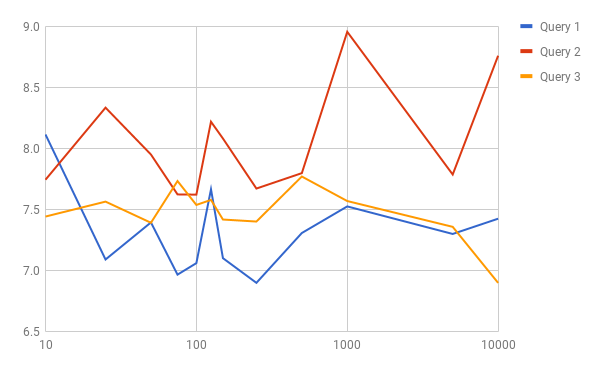
\includegraphics[width=.8\textwidth]{img/mongodb-query-size.png}
  \caption{MongoDB query size}
  \label{fig:mongodb-query-size}
\end{figure}

The horizontal axis in figure \ref{fig:mongodb-query-size} represents query size in the logarithmic scale.
The vertical axis represents the execution time of 10 000 iterations of the query in seconds.

All measured execution times fall roughly within 7 and 9 seconds, which means that the query execution time is constant for a varying query size in MongoDB

\begin{figure}
  \centering
  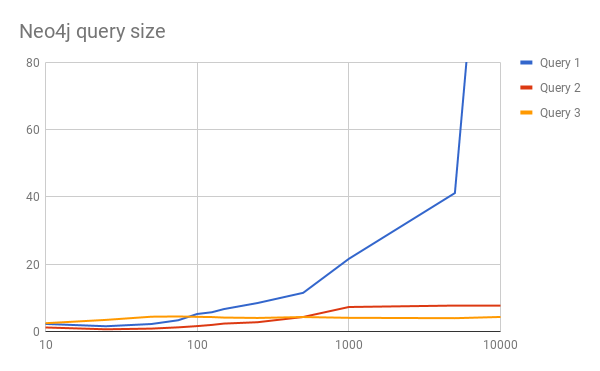
\includegraphics[width=.8\textwidth]{img/neo4j-query-size.png}
  \caption{Neo4j query size}
  \label{fig:neo4j-query-size}
\end{figure}

Neo4j however, renders a completely different result.
Figure \ref{fig:neo4j-query-size} plots out the execution time for the different queries running on the Neo4j graph database management system.
The first difference with MongoDB is already very apparent in iteration size: MongoDB can handle roughly 1000 times as many requests in the same execution time.
This is due to the fact that for every entity retrieved from the database, MongoDB only has to execute one request and retrieve one document, while Neo4j's inherent linked structure means that at least three entities have to be retrieved (event, subject and item).

Query 2 and query 3 remain constant, similar to their MongoDB equivalents.
Query 1 however, rises exponentially with query size.
This is not an expected result since a database index exists for the \texttt{created\_at} field on which the query orders.
However, for small, realistic values of query size this should not pose a problem.

\subsection{Iteration count}
\label{subsec:iteration-size}

The multiplication factor in these tests was set to 5000, similar to the previous tests.
Query size for all queries is 100.

Analogous to the previous test, query 4 was not included in the benchmark.

\begin{figure}
  \centering
  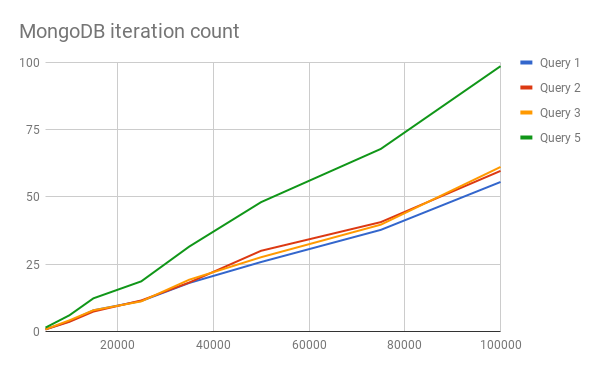
\includegraphics[width=.8\textwidth]{img/mongodb-iteration-count.png}
  \caption{MongoDB iteration count}
  \label{fig:mongodb-iteration-count}
\end{figure}

\begin{figure}
  \centering
  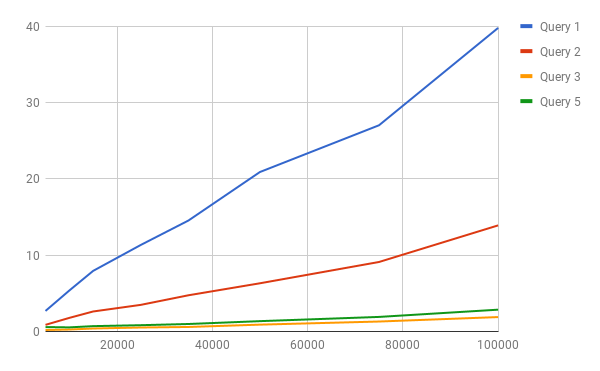
\includegraphics[width=.8\textwidth]{img/neo4j-iteration-count.png}
  \caption{Neo4j iteration count}
  \label{fig:neo4j-iteration-count}
\end{figure}

\section{Conclusion}
\label{sec:empirical-study-conclusion}

%   Language bindings: mongo yes, couch no, neo4j yes; impedance mismatch in mongo, especially related to polymorphism
